% /* cspell:disable */
\documentclass[a4paper,12pt]{book}

% import package
\usepackage{graphics}   % include graphics
\usepackage{float}      % h!

% figure
\usepackage{tikz}
\usepackage{pgfplots}
\usepackage{graphicx}
\usepackage{subcaption}

% page
\usepackage{fancyhdr}
\usepackage{setspace}
\usepackage{sectsty}

% math
\usepackage{amssymb}
\usepackage{amsmath}

% fancyhdr setting
\pagestyle{fancy}
\fancyhead{}
\fancyhead[LO]{\bfseries\rightmark}
\fancyhead[RO]{}
\fancyhead[RE]{\bfseries\leftmark}
\fancyhead[LE]{}

%table
\usepackage{multirow}
\usepackage{booktabs}
\usepackage{tabularx}
% page setting
\doublespacing
\allsectionsfont{\singlespacing}
\raggedbottom

% math symbols
\DeclareMathOperator*{\argmin}{arg\,min}
\DeclareMathOperator*{\argmax}{arg\,max}
\newcommand*\mean[1]{\overline{#1}}
\newcommand{\RN}[1]{
    \textup{\uppercase\expandafter{\romannumeral#1}}
}
%pdf plot
% \pgfplotsset{compat=1.15}
\begin{document}

% \tableofcontents

% %!TEX root = ../thesis.tex

\chapter{Introduction}

\section{Computational mechanics in civil engineering}

    \subsection{Mathematical model in mechanics}

    \subsection{Numerical method}

    \subsection{Computational mechanics in modern age}

\section{Current difficulties in numerical analysis}

    \subsection{Human effort on meshing}

    \subsection{Imperfection in geometric representation}

    \subsection{Lack of re-meshing scheme}

\section{Proposed approach}

\section{Research contribution}
    
    \subsection{Meshing based on CAD output in 2D and 3D}

    \subsection{High quality elements by Quad-tree}

    \subsection{Auto re-meshing based on error}

\section{Objectives and scope}

\section{Organization of the thesis}

\section{List of publications}


    % /* cspell:disable */
    % \begin{figure}[h!]
    %     \scalebox{1}{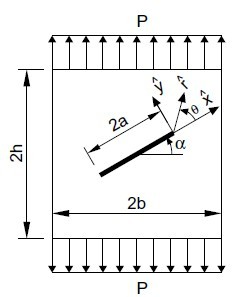
\includegraphics{chapter1/img/crackproblem.jpg}}
    % \end{figure}
    % /* cspell:enabled*/

% %!TEX root = ../thesis.tex

\chapter{Literature review}

\section{Overview of numerical methods}

    \subsection{Finite element method}

    \subsection{Boundary element method}

    \subsection{Isogeometric analysis}

\section{Scaled boundary finite element method}

\section{Approaches for meshing automation}

    \subsection{Initial Graphics Exchange Specification (IGES) file}

    \subsection{Non-Uniform Rational B-Spline (NURBS)}

\section{Conclusions}


%!TEX root = ../thesis.tex

% Isogeometric enhanced SBFEM in 2D
\section{Introduction}

\section{2D NURBS curves}
    \subsection{Numerical integrations}
\label{subsection:numerical_integration}
\paragraph{}
When computing the integrations in SBFEM % equation
    , numerical integrations tends to be overwhelmingly preferred over mathematical deduction. 
The reason behind lies in the flexibility of the numerical and that deduction of exact integrations scheme 
    to any given shape functions are not feasible. 
Due to the fact that the polynomials are adopted as the shape function, the numerical integrations methods 
    such as Legendre Quadrature or Gauss Quadrature provides possibility for an exact integration. 
An integration quadrature is normally defined as followed:
    \begin{equation}
        \int_{-1}^{1}
        f(x)dx 
        = \sum_{i=1}^n
        a_i f(x_i)
    \label{eq:numerical_integration}
    \end{equation}

\paragraph{}
Any given targeted polynomial function defined on $[-1,1]$ can be explicitly expressed as series.
A set of integration points $\left\{ x_1, x_2, \dots, x_n \right\} \in \left[-1,1\right]$ and the corresponding weight $\left\{ a_1, a_2, 
    \dots, a_n \right\} \in \mathbb{R}$ determined from the integration quadrature can be adopted to perform an exact integration
    on the given function.
\paragraph{}
Although shape functions used in NURBS are not polynomials, they can be separated into several spans where the function is a 
    rational polynomial. 
Based on this property, we are able to apply the numerical integration quadrature on each of these spans and achieve a reasonably 
    accurate result.
In other words, the NURBS curve with a knot vector of 
$[ 
    \underbrace{-1,-1,\dots,-1}_{p+1}, 
    u_0,\dots,u_n, 
    \underbrace{1,1,\dots,1 }_{p+1}
]$
can be integrated as
\begin{equation}
    \int_{-1}^{1} R(u) du = \int_{-1}^{u_0} R(u)du + 
                            \int_{u_0}^{u_1} R(u)du + \dots +
                            \int_{u_n}^1 R(u)du
\label{eq:numerical_integration_piecewise}
\end{equation}

\paragraph{}
Since the rational polynomials instead of the usual polynomials are utilized as the shape functions in NURBS, the difference between
    output from eq.~\ref{eq:numerical_integration_piecewise} and the analytical solution will be so large that can not be regarded as
    machine error.
Based on eq.~\ref{eq:rational_basis_function} we can conclude that the basis functions constructed by rational polynomials become
    non-rational if and only if the weight vector is identical i.e. $\left\{ w \right\} = \left[ 1,1,\dots,1 \right]$ after normalization.
That indicates the error of numerical integration will be decreased when the weight vector of the NURBS curves becomes more uniform as
    the basis functions are more close to non-rational polynomials.
In order to achieve this target, either or both of the knot insertion or the order elevation can be used.
\pagebreak
    \subsection{Surface traction}
\label{subsection:surface_traction}
\paragraph{}
In structural analysis, it is common to have boundary condition such as displacement constraints and applied load.
Due to the property of the NURBS that the control points are not necessarily on the curve, surface traction can not be
    applied by same method used in conventional numerical method like FEM or SBFEM.
A surface traction $\Phi$ can be regarded as Neumann boundary condition which can be expressed as
    \begin{equation}
        {F}=-\int_{\Gamma}
        [N]
        \Phi_n
        d\Gamma
    \label{eq:neumann_bc}
    \end{equation}
where $[N]$ describe the shape functions and $\Phi_n$ is the surface traction on the nodes.

\paragraph{}
As mentioned in \ref{subsection:numerical_integration}, numerical integration would be much more preferred over mathematical deduction
when the target function is an input. In the flavour of numerical integration, eq.~\ref{eq:neumann_bc} can be expressed as followed.
    \begin{equation}
        {F}=-\sum_{i=1}^n
        a_i
        [N(\xi_i)]
        \Phi_n
    \label{eq:neumann_bc_numerical}
    \end{equation}
Where $\xi_i$ is the integration points and $a$ is the weights,
$n$ is the number of integration points and different quadrature rule need different number to achieve a optimal accuracy.

\paragraph{}
It can be found that the term $[N(\xi_i)] \Phi_n$ is corresponding to $f(x)$ in eq.~\ref{eq:numerical_integration}.
In conventional FEM or SBFEM, $\Phi_n$ can be determined as the real values on the nodes because geometrically speaking,
    its shape function is interpolated from the given set of points.
In other words, all nodes that determine the shape function in traditional FEM or SBFEM must be on the interpolating function.
However, this is not the case in NURBS curves where it is the control points that play the same role as the nodes in existing
    shape function.
    % figure required
In NURBS curves, apart from the first and the last points, the control points are not necessarily on the curves.
This prevent us from adopting the physical value on the nodes as $\Phi_n$ in eq.~\ref{eq:neumann_bc_numerical}.
Instead, a set of ``control stress'' $\Phi_c$, the control points of another NURBS curve that represent the surface traction
    geometrically, need to be determined as \footnote{$\argmin_x f(x) = \left\{
        x | x \in S \wedge \forall y \in S : f(y) \geq f(x)
    \right\}$}
    \begin{equation}
        \Phi_c = \argmin_{\Phi_c}
            \frac{1}{2}
            \int_{-1}^1
            \|
                \Phi(\xi)-
                    \left[ N(\xi) \right]
                    \Phi_c
            \|^2
            d\xi            
    \label{eq:surface_traction_fitting}
    \end{equation}

\paragraph{}
It means that ``control stress'' $\Phi_c$ describe a minimum mean squared error between surface traction NURBS curve and the real
    traction $\Phi$.
One of the simplest mathematical method to determine $\Phi_c$ will be least square method.
Given the fact that the shape functions of this NURBS curve will be the same as that describe the geometry, $\left[ N(\xi) \right]$
    can be considered as known.
By selecting $n$ sample points over the domain of the $\Phi$, eq.~\ref{eq:surface_traction_fitting} can be rewrite as
    \begin{equation}
        \Phi_c = \argmin_{\Phi_c}
            \frac{1}{n}
            \sum_{i=1}^n
            \|
                \Phi(\xi_i)-
                    \left[ N(\xi_i) \right]
                    \Phi_c
            \|^2
    \label{eq:surface_traction_fitting_discrete}
    \end{equation}
Then ``control stress'' $\Phi_c$ can be solved by least square as
    \begin{equation}
        \Phi_c= \left(
            \left[ N(\xi) \right] ^T
            \left[ N(\xi) \right]
        \right)^{-1}
        \left[ N(\xi) \right]^T
        \Phi(\xi)
    \end{equation}
and eq.~\ref{eq:neumann_bc_numerical} in the case where NURBS is in use can be rewrite as
    \begin{equation}
        {F}=-\sum_{i=1}^n
        a_i
        [N(\xi_i)]
        \Phi_c
    \label{eq:neumann_bc_numerical_NURBS}
    \end{equation}
\pagebreak
    
\section{Formulation of SBFEM}

\section{NURBS enhanced SBFEM}
    \subsection{Displacement interpolation}
\paragraph{}
Another difference between it with conventional FEM or SBFEM lies in the post processing.
After solving the partial differential equation numerically, the displacements on the nodes will be one of the output in
    the traditional method.
However, similar to what is discussed in \ref{subsection:surface_traction}, NURBS curves are defined by the control points
    that are not geometrically located on the curves.
As a consequence, not only the input such as surface traction need to be translated into a NURBS-like representation, the
    output such as the displacements will be the dummy values on the control points as well, or ``control displacements''
    $\left\{ u_c \right\}$.
Dislike that in the traditional method, the ``control displacements'' do not have any physical meaning. It can only be used
    to interpolate the real displacements within its span.

\begin{equation}
    \left\{ u \right\}=
    \sum_{i=0}^n
    R(u) \left\{u^{(N)}\right\}
\label{eq:displacement_interpolation}
\end{equation}
\pagebreak

\section{Numerical examples}
    \subsection{Cantilever beam}
\paragraph{}
A two-dimensional cantilever beam subjected to a parabolic shear load at the free end is examined as shown
in fig.~\ref{fig:cantilever_beam_geo_bc}.
    \begin{figure}[h!]
    \centering
        \scalebox{0.8}{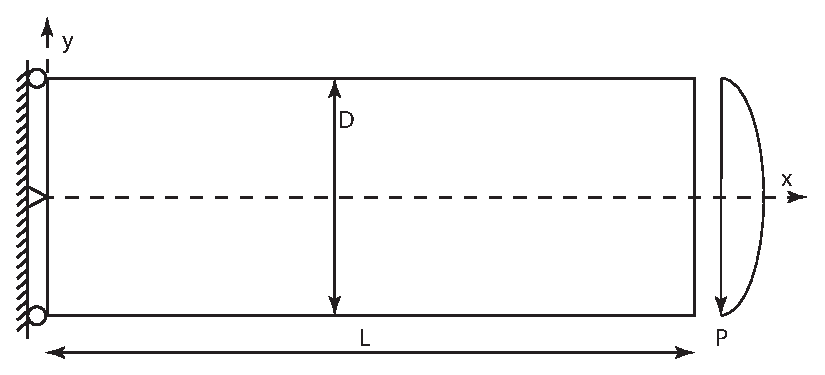
\includegraphics{isogeometric_sbfem/images/cantilever_beam_geo_bc.eps}}
        \caption{ Cantilever beam: Geometry and boundary conditions.}
        \label{fig:cantilever_beam_geo_bc}
    \end{figure}

The geometry is: length $L=8m$, height $D=4m$.
The material properties are: Young’s modulus $E$ = $3 \times 10^7 N/m^2$ , Poisson’s ratio $ν=0.25$.
The parabolic shear force is $P$ = $250 N$.
The exact solutions for the displacements are given by \cite{Aug2008}:
    \begin{equation}
        \begin{aligned}
            u(x,y) &= 
                \frac{Py}{6 \mean{E} I}
                \left[
                    \left(
                        6L-3x
                    \right)x
                    +\left(
                        2+ \mean{v}
                    \right)\left(
                        y^2-\frac{D^2}{4}
                    \right)
                \right]
            \\
            v(x,y) &=  
                -\frac{P}{6 \mean{E} I}
                \left[
                    3 \mean{v} y^2 \left(
                        L-x
                    \right)+
                    \left(
                        4+5 \mean{v}
                    \right)\frac{D^2x}{4}+
                    \left(
                        3L-x
                    \right)x^2
                \right]        
        \end{aligned}
    \label{eq:cantilever_beam_displacement_solution}
    \end{equation}

where $I=D^3/12$ is the moment of inertia, $\mean{E}=E$, $\mean{v}=v$ and $\mean{E}=E/(1-v^2)$, $\mean{v}=v/(1-v)$ for plane
    stress and plane strain condition respectively.
The stress $\sigma$ can be expressed as \cite{Aug2008}
    \begin{subequations}
    \begin{align}
        \sigma_{xx} &= \frac{P(L-x)y}{I} \\
        \sigma_{yy} &= 0 \\
        \tau_{xy} &= -\frac{P}{2I} \left[
            \frac{D^2}{4} - y^2
        \right]
    \end{align}
    \label{eq:cantilever_beam_stress_solution}
    \end{subequations}

The strain energy can be derived from eq.~\ref{eq:cantilever_beam_stress_solution} and eq.~\ref{eq:cantilever_beam_displacement_solution} as
    \begin{equation}
        \frac{1}{2} \left(
            \frac{D^3 L^3 P^2}{36EI^2} + 
            \frac{D^5LP^2(1+v)}{60EI^2}
        \right)
    \label{eq:cantilever_beam_energy_solution}
    \end{equation}

\paragraph{}
In this example, rigid body motion is constrained by fixing 3 DOF on the left edge of the beam.
$u_x=0$ for points at $(0,-D/2)$ and $(0,D/2)$ and $u_y =0$ for point at $(0,0)$.
Stress from analytical solution in eq.~\ref{eq:cantilever_beam_stress_solution} are applied on the boundary.

\paragraph{}
From the description in \ref{subsection:surface_traction}, the expression of the surface traction must be transformed into
    NURBS-like representation before the stress can be applied on the nodes.
Although least square is introduced to solve for the ``control stress'' $\Phi_c$, the control points that describe a second
    order function as surface traction in this example can be solved mathematically.
Assume the knot vector is evenly spaced and the shape function is in second order, i.e. knot vector $K=[0,0,0,1,1,1]$.
Weight vector will be uniform because only the straight line is being interpolated, i.e. weight vector $w=[1,1,1]$.
Three basis function used in B-Spline will be
    \begin{equation}
    \begin{aligned}
        N_1 & = (1-u)^2 \\
        N_2 & = 2u(1-u) \\
        N_3 & = u^2
    \end{aligned}
    \end{equation}

With the given targeted parabola as $y=ax^2+bx+c,x \in [0,1]$, the generalized control points for the NURBS curve will be
    \begin{equation}
        P= \begin{bmatrix}
            P_x \\
            P_y
        \end{bmatrix} = \begin{bmatrix}
            0 & m & 1 \\
            c & n & a+b+c
        \end{bmatrix}
    \end{equation}

where $m$ and $n$ are unknowns for the second control point.
B-spline curve $C=[N][[P]$ then can be expressed as in parametric form as
    \begin{equation}
        \left\{
        \begin{aligned}
            x &= 2u(1-u)m + u^2 \\
            y &= c(1-u)^2 + 2u(1-u)n + (a+b+c)u^2
        \end{aligned}
        \right.
    \label{eq:parabola_fitting_parametric}
    \end{equation}

After substituting eq.~\ref{eq:parabola_fitting_parametric} into $y=ax^2+bx+c$, we then have the system of equations as
    \begin{equation}
        \begin{bmatrix}
            0 \\
            0 \\
            2c - 2n +a +b \\
            2n - 2c \\
            c
        \end{bmatrix} = 
        \begin{bmatrix}
            4am^2-4am+a \\
            -8am^2 + 4am \\
            4am^2 -2bm +b \\
            2bm \\
            c
        \end{bmatrix}
    \end{equation}

$m$ and $n$ then can be solved as
    \begin{equation}
        \left\{
        \begin{aligned}
            m &= \frac{1}{2} \\
            n &= \frac{b+2c}{2}
        \end{aligned}
        \right.
    \end{equation}

\paragraph{}
The numerical convergence of the relative error in the displacement norm and the relative error in the energy norm are
    shown in fig.~\ref{fig:cantilever_beam_convergence} for various order of NURBS basis functions with refinement.
Fig.~\ref{fig:cantilever_beam_convergence} also shows the error in the displacement norm when quadratic Lagrange shape
    functions are used along each edge within the scaled boundary formulation.
It can be observed that NURBS basis functions yield superior accuracy when compared to Lagrange basis functions of the
    same order.
It is seen that as the order of the shape functions is increased, the error decreases while the convergence rate increases.

\begin{figure}
    \begin{subfigure}[b]{1\linewidth}
        \centering
        \scalebox{0.7}{
            % This file was created by matlab2tikz v0.4.6 running on MATLAB 8.2.
% Copyright (c) 2008--2014, Nico Schlömer <nico.schloemer@gmail.com>
% All rights reserved.
% Minimal pgfplots version: 1.3
% 
% The latest updates can be retrieved from
%   http://www.mathworks.com/matlabcentral/fileexchange/22022-matlab2tikz
% where you can also make suggestions and rate matlab2tikz.
% 
\begin{tikzpicture}

\begin{axis}[%
width=4.52083333333333in,
height=3.5146875in,
scale only axis,
xmode=log,
xmin=10,
xmax=1000,
xminorticks=true,
xlabel={Total DOF},
ymode=log,
ymin=1e-05,
ymax=1,
yminorticks=true,
ylabel={Error},
title={l2l Displacement  Error},
legend style={draw=black,fill=white,legend cell align=left}
]
\addplot [color=blue,solid,mark=square,mark options={solid}]
  table[row sep=crcr]{
20	0.223473837	\\
40	0.0493	\\
80	0.011281049	\\
160	0.00266076	\\
};
\addlegendentry{1st order};

\addplot [color=black!50!green,solid,mark=o,mark options={solid}]
  table[row sep=crcr]{
20	0.067810872	\\
40	0.003190002	\\
80	0.000250473	\\
160	2.27e-05	\\
};
\addlegendentry{2nd order};

\addplot [color=red,solid,mark=+,mark options={solid}]
  table[row sep=crcr]{
20	0.0713	\\
40	0.00707	\\
80	0.000688	\\
160	8.85e-05	\\
};
\addlegendentry{LNGL 2nd order};

\end{axis}
\end{tikzpicture}%
        }
        % \label{fig:cantilever_beam_displacement_convergence}
        \caption{the relative error in displacement norm $(L^2)$}
    \end{subfigure}
    
    \begin{subfigure}[b]{1\linewidth}
        \centering
        \scalebox{0.7}{
            % This file was created by matlab2tikz v0.4.6 running on MATLAB 8.2.
% Copyright (c) 2008--2014, Nico Schlömer <nico.schloemer@gmail.com>
% All rights reserved.
% Minimal pgfplots version: 1.3
% 
% The latest updates can be retrieved from
%   http://www.mathworks.com/matlabcentral/fileexchange/22022-matlab2tikz
% where you can also make suggestions and rate matlab2tikz.
% 
\begin{tikzpicture}

\begin{axis}[%
width=4.52083333333333in,
height=3.5146875in,
scale only axis,
xmode=log,
xmin=10,
xmax=1000,
xminorticks=true,
xlabel={Total DOF},
ymode=log,
ymin=0.001,
ymax=1,
yminorticks=true,
ylabel={Error},
title={l2l Strain Energy  Error},
legend style={draw=black,fill=white,legend cell align=left}
]
\addplot [color=blue,solid,mark=square,mark options={solid}]
  table[row sep=crcr]{
20	0.701427116670007	\\
40	0.417133072292284	\\
80	0.228254244210267	\\
160	0.119582607431014	\\
};
\addlegendentry{1st order};

\addplot [color=black!50!green,solid,mark=o,mark options={solid}]
  table[row sep=crcr]{
20	0.180496573374677	\\
40	0.02575787258296	\\
80	0.0046690470119715	\\
160	0.0010295630140987	\\
};
\addlegendentry{2nd order};

\addplot [color=red,solid,mark=+,mark options={solid}]
  table[row sep=crcr]{
20	0.304275389	\\
40	0.065	\\
80	0.014502273	\\
160	0.003385053	\\
};
\addlegendentry{LNGL 2nd order};

\end{axis}
\end{tikzpicture}%
        }
        % \label{fig:cantilever_beam_energy_convergence}
        \caption{the relative error in the energy norm}
    \end{subfigure}
\label{fig:cantilever_beam_convergence}
\caption{Bending of thick cantilever beam: Convergence results}
\end{figure}
\pagebreak
\section{Conclusions}

% %!TEX root = ../thesis.tex

\chapter{Quad-tree mesh and auto refinement in 2D analysis based on error}

\section{Introduction}

\section{CAD output in 2D}

\section{NURBS utilization}

    \subsection{Distance function}

    \subsection{Finding intersections}

    \subsection{Optimization}

\section{Quad-tree structure}

\section{Conclusions}
% %!TEX root = ../thesis.tex

\chapter{Adaptivity}

\section{Introduction}

\section{Lambda error indicator in SBFEM}

\section{Artificial neural network}

    \subsection{Learning algorithms}

    \subsection{Optimization algorithms}

        \subsubsection{Quasi-Newton methods}

        \subsubsection{Stochastic gradient descent}

        \subsubsection{Stochastic gradient-based optimizer proposed by Kingma, Diederik, and Jimmy Ba}

    \subsection{Activation function}

        \subsubsection{Identity}

        \subsubsection{Logistic}

        \subsubsection{Tanh}

        \subsubsection{Rectified linear unit function}

    \subsection{Learning rate}

    \subsection{Backpropagation algorithm}

\section{Multi-layer perceptron}

\section{Conventional neural network(not decided yet)}

\section{Numerical examples}

\section{Conclusions}


% %!TEX root = ../thesis.tex

\chapter{Isogeometric enhanced SBFEM in 3D}

\section{Introduction}

\section{Formulation of SBFEM in 3D}

\section{CAD output in 3D}

\section{NURBS in 3D}

    \subsection{Surfaces division}

    \subsection{Finding projection}

    \subsection{Optimization using matrix representation}

\section{Numerical examples}

\section{Conclusions}
% %!TEX root = ../thesis.tex

\chapter{Conclusions and recommendation}

% reference
\pagebreak
\bibliographystyle{plain}
\addcontentsline{toc}{chapter}{Bibliography}
\bibliography{ref}


\end{document}